\section{The Seven}

\vspace{4mm}

\begin{center}
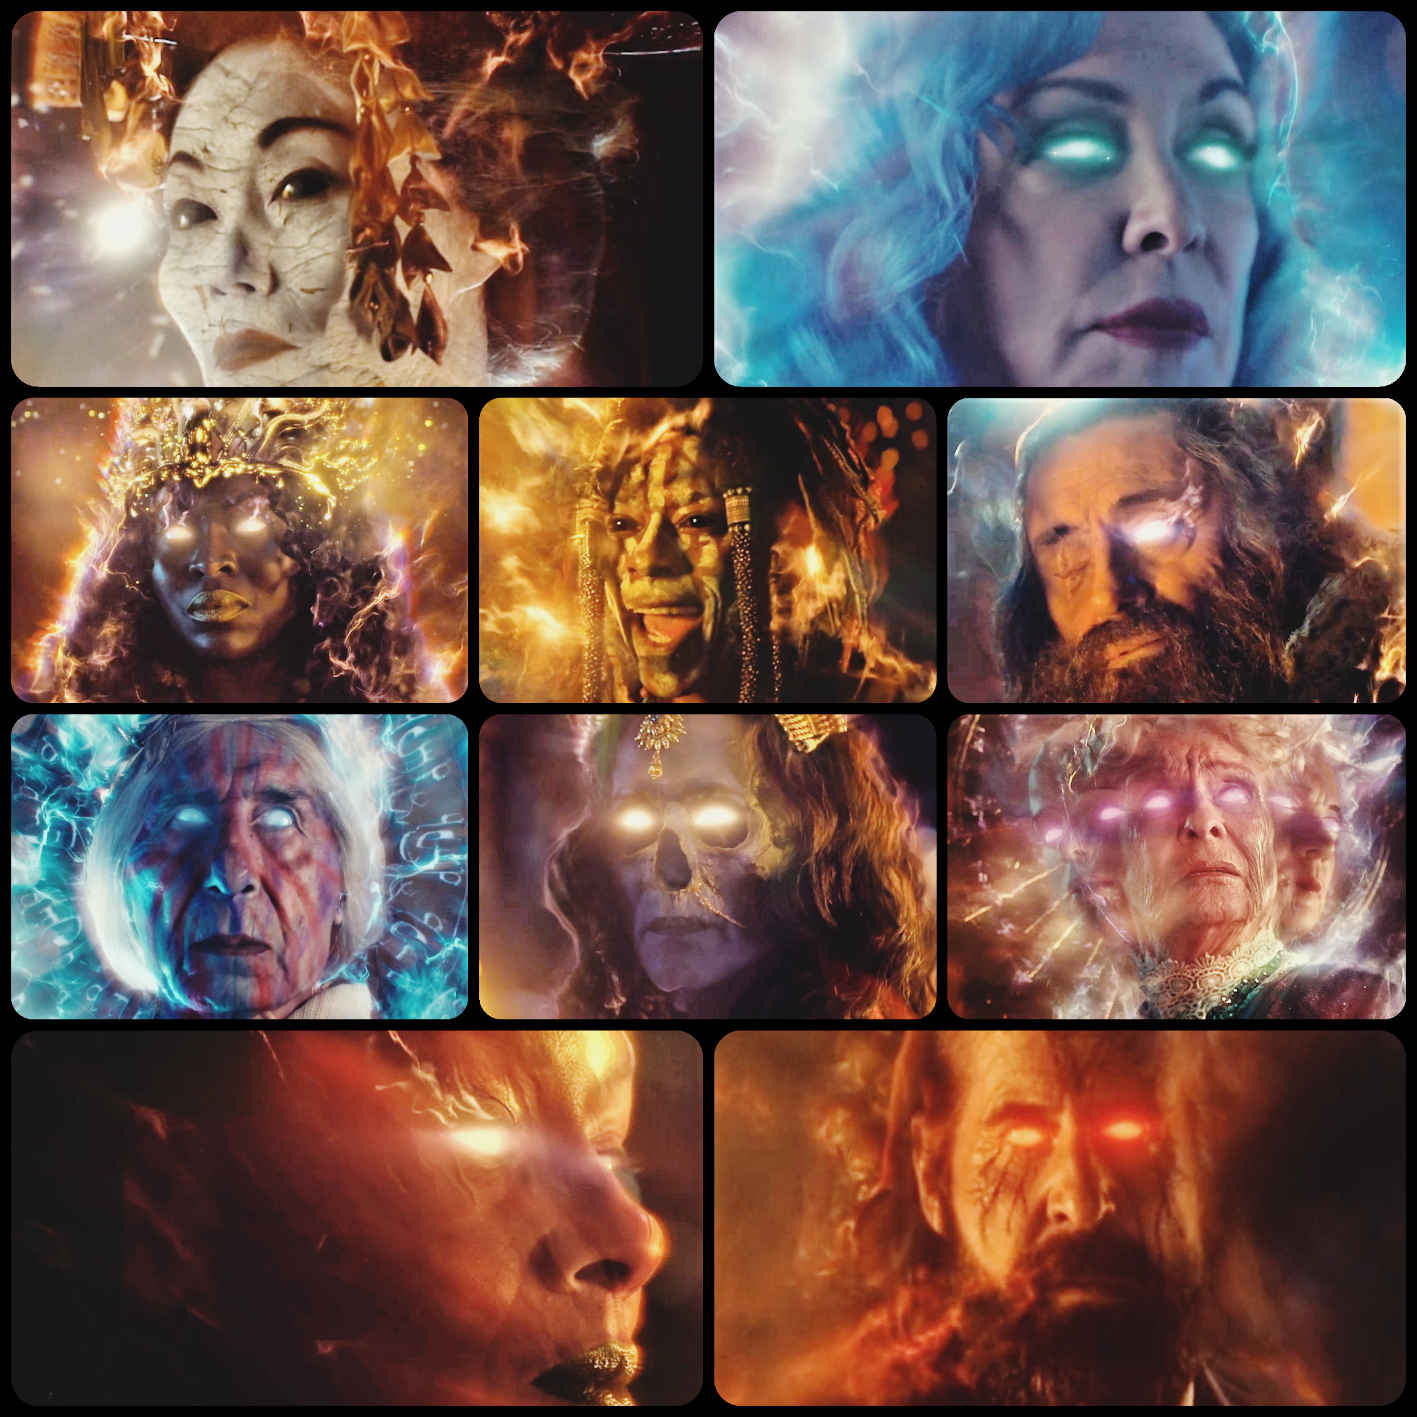
\includegraphics[width=80mm]{./content/img/theGods.jpg}
\begin{figure}[h]
\end{figure}
\end{center}

\subsection*{Details} 

\vspace{2mm}

There are seven gods:

\subsubsection{Lathor - The Mother and Father, The Horizon}

\vspace{2mm}

The first among equals. Goodness, Faith, Leadership, Family

Lathor rarely acts directly in the epic tales told of the gods engaging in their grand wars. Rather, the tales always start with Lathor tasking the other gods with going to a particular location, destroying a particular evil creature or finding a particular item. Then, at the end of tale, when the battle is won, usually with a bitter price paid, Lathor returns, to deliver the moral of the story and teach the relevant lesson.

\subsubsection{Elledun - The Lantern-Bearer, The Rising Sun}

\vspace{2mm}

Hope, Light Against the Darkness, Agriculture, Travellers

Followers of Elledun often build roadside shrines, marked by a small candle, protected from the elements with a glass cover. Weary travellers will find supplies contained within, and are expected to contribute in kind when well-stocked.

\subsubsection{Belladon - The Open-Handed, The Crystal Spring}

\vspace{2mm}

Charity, Giving to Those in Need, Forgiveness, The Home


\subsubsection{Hemotate - The Book-Bearer, The Tree in the Storm}

\vspace{2mm}

Justice, Fairness, Karma, Scholarly Pursuits

Devotees of Hemotate make a habit of claiming that by the time Hemotate arrived to a battle, the day was already won. Using preparation, research, and their enemies weaknesses, they often found no need for weapons. The forces of darkness brought their own undoing, and Hemotate was able to pick at the right threads to unravel their plans.

\subsubsection{Vathos - The Shield-Bearer, The Weathered Rock}

\vspace{2mm}

Fortitude, Strength Against Adversity, Undergoing Punishment

In legends, Vathos would enter battle against the forces of darkness wielding only a shield. With each blow that landed upon him, his strength grew. He would stand in the midst of battle, taking blow after blow without striking back until, when the moment came, he would fell whole armies with a single punch.

\subsubsection{Novetta- The Arms-Bearer, The Consuming Fire}

\vspace{2mm}

Valor, Fighting Against Evil, Vengeance

Novetta eschewed armour, and would enter battle armed only with her bastard sword, Fynyr. It is said that Fynyr was sharp enough to sever the connection between an enemies body and their soul.

\subsubsection{Matreus - The Standard-Bearer, The Tower on the Hill}

\vspace{2mm}

Loyalty, Conviction

Matreus was said to be deaf and blind, and fought valiantly in battle, never knowing whether his compatriots were standing firm or had turned and fled long ago. Seen as a lonely figure, but one that is never discouraged by that fact.

His most ardent followers tend to live in isolation, meeting only to share wisdom and scriptures. They believe that a faith that is tested most often, and which still holds, is the truest, and that strength never used is no strength at all.

\subsubsection{Synne - The Horseman, The Buried Spire}

\vspace{2mm}

???

While some people favour one god in particular, this is not common, and is viewed with suspicion by some in the church.

\subsection*{The God's PLace in the World}

More frequently, people have a few of the gods which, when taken in combination, express their outlook. For example, many Arbiters favour a combination of Hemotate and Novetta, representing their drive to punish lawbreakers, whereas many Pastors favour a combination of Elledun and Belladon, in the hope that they may spread the light of their faith to those in their community.

A sailor going to sea may pray to Elledun and Matreus when setting out on their journey, so that they may stay true to their path and not get lost, but pray to Belladon and Vathos when their ship is caught in a storm, to gift them with the strength to carry on.

Demons do the torturing
Devils din the book keeping
Where the fuck are the Gods?

Turns out that they have all fucked off on holiday leaving the world to fend for itself and be abused by the Church. Re-connecting the world to the internet again will allow the software to update and the Gods to return with all their awesome power.


\begin{DndSidebar}{Fallen Twin}
 dfhgsfdghfsgh
\end{DndSidebar}

\smallskip

\bigskip

%\begin{DndSidebar}[float=!b]{Behold the DndSidebar!}
 %dfhgsfdghfsgh
%\end{DndSidebar}

\clearpage